\begin{figure}[!ht]
	\centering
	\setlength{\resLen}{1.4in}
	\addtolength{\tabcolsep}{0pt}
	\begin{tabular}{ccc}
		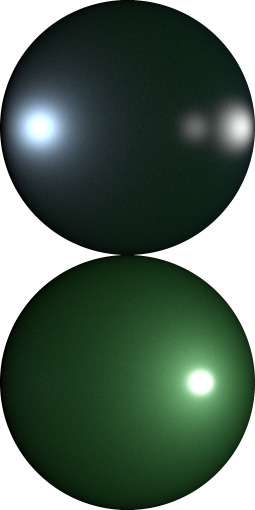
\includegraphics[width=\resLen]{layeredbsdf/validations/lobe_bsdf/bsdf_sample_all.jpg} &
		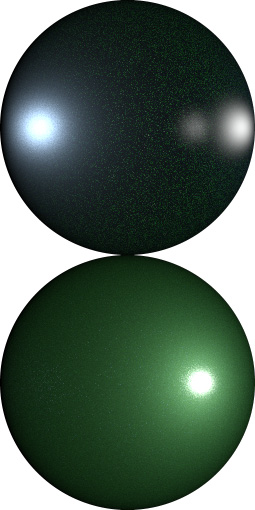
\includegraphics[width=\resLen]{layeredbsdf/validations/lobe_bsdf/bsdf_eval_uni_all.jpg} &
		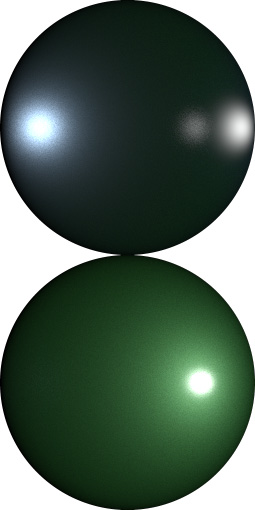
\includegraphics[width=\resLen]{layeredbsdf/validations/lobe_bsdf/bsdf_eval_bi_all.jpg} \\
		Ground truth &
		Our unidir. &
		Our bidir. \\
	\end{tabular}
	\caption[Outgoing lobes of a layered BSDF]{\label{fig:layeredbsdf:lobes}
		\textbf{Outgoing lobes of a layered BSDF} (reflection and transmission) visualized as projected hemispheres. \textbf{Left:} ground truth computed by sampling and binning the light paths. \textbf{Middle:} Our unidirectional estimator. \textbf{Right:} Our bidirectional estimator (same time).
	}
\end{figure}